\chapter{YOLO Instance Segmentation}\label{ch:yolo}

\section{Introduction}\label{sec:yolo-intro}
The YOLO family of models (``you only look once'') began as fast object detectors~\citep{yolo}. The
segmentation versions in the Ultralytics library~\citep{ultralytics} add a mask to each detected box
using the prototype idea of YOLACT~\citep{yolact}, which we introduced briefly in
Section~\ref{sec:paradigms-decoders}. We used two of these models: \keyterm{YOLO11m-seg}, with about
22 million parameters, and \keyterm{YOLOv8l-seg}, with about 46 million.\footnote{YOLOv8 and
YOLO11 are successive releases of the Ultralytics family of models. The letters m and l denote the
medium and large variants, and the suffix \texttt{-seg} denotes the segmentation version.} Both come pretrained on
COCO, whose 80 everyday classes contain nothing resembling a solar filament, and we fine-tuned both
with a single class.

This family carried our public score from 0.32 to 0.39, and it taught us most of what we know about
the problem. In Section~\ref{sec:yolo-arch} we describe how YOLO produces masks and how it is
trained. Section~\ref{sec:yolo-exp002} reports our first instance model, and
Section~\ref{sec:yolo-resolution} shows that simply running it at the native resolution helped a
great deal. Section~\ref{sec:yolo-erosion} describes the discovery that its masks were
systematically too wide, and traces the cause. Section~\ref{sec:yolo-retrain} follows our attempts
to retrain the model properly at the native resolution, and Section~\ref{sec:yolo-lessons}
summarises what the YOLO models could and could not do.

\section{A detector that also draws masks}\label{sec:yolo-arch}
Figure~\ref{fig:yolo-arch} shows the flow of data through a YOLO segmentation model. A convolutional
\keyterm{backbone} computes feature maps at three strides, 8, 16 and 32 pixels. A \keyterm{neck}
then mixes these maps top-down, as in a feature pyramid network~\citep{lin2017fpn}, and again
bottom-up, as in a path aggregation network~\citep{liu2018panet}, so that every scale has access to
both fine detail and wide context. After the neck, two things happen in
parallel.
\begin{itemize}[leftmargin=*,itemsep=2pt]
\item A \keyterm{detection head} runs at every location of every scale. Each location predicts a
box, a confidence score, and a vector of $k=32$ \keyterm{mask coefficients}.
\item A \keyterm{prototype branch} turns the finest feature map into $k=32$ \keyterm{prototype} maps
$P_1,\dots,P_{32}$, each of which covers the whole image at a quarter of the input resolution.
\end{itemize}
After non-maximum suppression~\citep{neubeck2006} has removed duplicate boxes, each surviving detection $d$, with
coefficients $\mathbf{c}_d$ and box $B_d$, receives the mask
\begin{equation}
m_d(\mathbf{u}) = \mathbf{1}\!\left[\,\sigmoid\!\Big(\textstyle\sum_{j=1}^{k} c_{dj}\,P_j(\mathbf{u})\Big) > 0.5\,\right]
\cdot \mathbf{1}[\mathbf{u}\in B_d],
\label{eq:yolo-mask}
\end{equation}
where $\mathbf{u}$ ranges over pixel positions and $\mathbf{1}[\cdot]$ equals 1 when its condition
holds and 0 otherwise. The prototypes are shared by every detection in the image, so what
distinguishes one detection's mask from another's is only its 32 mixing weights and its box.

\begin{figure}[t]
\centering
\begin{tikzpicture}[
  stage/.style={box=#1, text width=1.72cm, minimum height=1.15cm, font=\sffamily\scriptsize,
                execute at begin node={\hyphenpenalty=10000}}]
  \node[stage=inkmuted] (img) at (0,0) {photograph, resized to the input size};
  \node[stage=vizblue] (bb) at (2.35,0) {backbone: features at strides 8, 16, 32};
  \node[stage=vizblue] (neck) at (4.7,0) {neck: feature pyramid, top-down and bottom-up};
  \node[stage=vizblue] (det) at (7.25,0) {detection head: per location a box, a score and 32 coefficients};
  \node[stage=vizblue] (nms) at (10.1,0) {confidence floor and non-maximum suppression};
  \node[stage=vizaqua] (proto) at (7.25,-1.9) {prototype branch: 32 maps at 1/4 of the input};
  \node[stage=vizorange] (mix) at (10.1,-1.9) {mask $=\sigmoid(\mathbf{c}_d^{\top}\mathbf{P})$, cut to the box, threshold 0.5};
  \draw[flow] (img) -- (bb); \draw[flow] (bb) -- (neck); \draw[flow] (neck) -- (det);
  \draw[flow] (det) -- (nms); \draw[flow] (neck.south) |- (proto.west);
  \draw[flow] (proto) -- (mix); \draw[flow] (nms) -- (mix);
\end{tikzpicture}
\caption{YOLO segmentation. The detection head finds objects and gives each one 32 mixing
coefficients; the prototype branch predicts 32 whole-image maps once; and each detection's mask is
the sigmoid of its own mixture of the shared maps, cut to its box.
\drawnin{book/chapters/ch07\_yolo.tex}}
\label{fig:yolo-arch}
\end{figure}

\subsection{Prototypes as a basis}\label{sec:yolo-prototypes}
Equation~\eqref{eq:yolo-mask} says that every mask is a thresholded linear combination of the same
32 images. It is helpful to think of the prototypes as a \keyterm{basis}, like the sines and cosines
of a Fourier series, from which each detection builds its own shape. The network learns the basis,
so the prototypes become whatever shapes are most useful for the training data, such as edges at
various orientations, blobs, and gradients across the image. Figure~\ref{fig:yolo-proto} sketches
the idea.

\begin{figure}[t]
\centering
\begin{tikzpicture}[
  sq/.style={minimum size=1.15cm, draw=inkmuted, line width=0.5pt, inner sep=0pt},
  op/.style={font=\sffamily\small, text=inksecondary}]
  \shade[left color=white, right color=vizblue!80] (0,0) rectangle (1.15,1.15);
  \draw[inkmuted, line width=0.5pt] (0,0) rectangle (1.15,1.15);
  \shade[top color=vizblue!80, bottom color=white] (1.75,0) rectangle (2.9,1.15);
  \draw[inkmuted, line width=0.5pt] (1.75,0) rectangle (2.9,1.15);
  \begin{scope}
    \clip (3.5,0) rectangle (4.65,1.15);
    \fill[white] (3.5,0) rectangle (4.65,1.15);
    \draw[vizblue!70, line width=9pt, line cap=round, opacity=0.8] (3.35,0.15) -- (4.8,1.0);
  \end{scope}
  \draw[inkmuted, line width=0.5pt] (3.5,0) rectangle (4.65,1.15);
  \node[op] at (0.575,-0.3) {$\times\,0.9$};
  \node[op] at (2.325,-0.3) {$\times\,(-0.6)$};
  \node[op] at (4.075,-0.3) {$\times\,1.8$};
  \node[op] at (1.45,0.575) {$+$};
  \node[op] at (3.2,0.575) {$+$};
  \node[op] at (5.2,0.575) {$+\;\cdots$};
  \node[op] at (5.95,0.575) {$\Rightarrow$};
  % the mixed logit map
  \begin{scope}
    \clip (6.4,0) rectangle (7.55,1.15);
    \shade[left color=vizblue!8, right color=vizblue!35] (6.4,0) rectangle (7.55,1.15);
    \draw[vizblue, line width=6pt, line cap=round, opacity=0.9] (6.25,0.2) -- (7.7,1.0);
  \end{scope}
  \draw[inkmuted, line width=0.5pt] (6.4,0) rectangle (7.55,1.15);
  \node[op] at (8.1,0.575) {$\Rightarrow$};
  % thresholded and cut to the box
  \fill[gridline!50] (8.6,0) rectangle (9.75,1.15);
  \begin{scope}
    \clip (8.75,0.12) rectangle (9.6,1.03);
    \draw[vizorange, line width=5pt] (8.45,0.2) -- (9.9,1.0);
  \end{scope}
  \draw[inkprimary, dashed, line width=0.5pt] (8.75,0.12) rectangle (9.6,1.03);
  \draw[inkmuted, line width=0.5pt] (8.6,0) rectangle (9.75,1.15);
  \node[note] at (2.325,1.45) {three of the 32 shared prototypes};
  \node[note] at (6.975,1.45) {mixture (logits)};
  \node[note] at (9.175,1.45) {sigmoid, box, 0.5};
\end{tikzpicture}
\caption{A schematic of mask assembly in YOLO segmentation. A detection's 32 coefficients weight the
shared prototype maps. The weighted sum is a map of logits, which is passed through a sigmoid, cut to
the detection's box (dashed) and thresholded. The prototype shapes drawn here are illustrative, not
learned ones. \drawnin{book/chapters/ch07\_yolo.tex}}
\label{fig:yolo-proto}
\end{figure}

This design has a cost that matters for filaments. The basis has only 32 members, and it lives at a
quarter of the input resolution. A filament is thin and curved, and the prototypes are smooth maps
shared with every other filament in the photograph, so the mixture must carve a narrow ridge out of
a few broad shapes. Before the retraining experiments of Section~\ref{sec:yolo-retrain}, we wrote
down a test of this concern: if a properly trained model at the native resolution still failed to
improve on validation, then the 32-prototype basis would be the limiting factor. As we explain in
Section~\ref{sec:yolo-lessons}, the test never came out clearly enough to settle the question.

\subsection{How YOLO is trained}\label{sec:yolo-training}
During training, each annotated filament must be assigned to a few locations of the detection head,
which are then trained to detect it. Ultralytics uses a \keyterm{task-aligned
assigner}~\citep{feng2021tood,ultralytics}. For each annotated object it considers the locations whose centres
lie inside the object's box, and it scores each location by the alignment metric
\begin{equation}
t = s^{\alpha}\,u^{\beta},
\end{equation}
where $s$ is the score that the location currently assigns to the object's class and $u$ is the IoU
between the location's predicted box and the object's box. A location is therefore a good candidate
only if it both recognises the object \emph{and} localises it well. With the library's default
values, $\alpha=0.5$ and $\beta=6$, the ten best-aligned locations become positives for that object.

The loss has four parts. A binary cross-entropy for the class score is computed at every location,
with a soft target derived from the alignment metric at the positive locations and zero elsewhere.
Each positive location also receives a box loss based on the complete IoU
(CIoU)~\citep{zheng2020diou} between its predicted box and the object's box, a distribution focal
loss (DFL)~\citep{li2020gfl} on the positions of the four box edges, and a \keyterm{mask loss}. The mask loss is the per-pixel binary cross-entropy between the
unthresholded mask of Equation~\eqref{eq:yolo-mask} and the annotated mask, counted only inside the
object's box and normalised by the box's area. The mask loss is where the pixel-level supervision
lives, and three of the lessons of this chapter concern its resolution.

During training, Ultralytics reports the model's progress as \keyterm{mean average precision}
(mAP)~\citep{everingham2010,coco}. Average precision integrates precision over all confidence thresholds, so it measures how well
the model \emph{ranks} its candidates. PQ, by contrast, scores a single emitted set of masks at a
single threshold. The two can disagree, and during this project they often did: the mAP of a
checkpoint told us little about its PQ until we had swept its threshold and scored it.

\section{The first instance model}\label{sec:yolo-exp002}
In exp002 we fine-tuned YOLO11m-seg at an input size of $1280\times1280$ for 149 epochs. A time
budget of 8.5 hours stopped the run while its mask mAP50 was still rising over the last thirty
epochs. It reached a mask mAP50 of 0.709 and scored 0.32 on the public leaderboard, six hundredths
above the dense models. As we saw in Section~\ref{sec:paradigms-stop}, the gain came from
recognition.

We then swept the confidence threshold over seven values and the minimum area over three values. The
best settings were:
\begin{center}\small
\begin{tabular}{@{}cccccccc@{}}
\toprule
confidence & min area & PQ & SQ & RQ & TP & FP & FN \\
\midrule
0.30 & 300 & \textbf{0.3736} & 0.643 & 0.581 & 721 & 437 & 604 \\
0.25 & 150 & 0.3714 & 0.643 & 0.578 & 751 & 523 & 574 \\
0.40 & 150 & 0.3657 & 0.648 & 0.565 & 626 & 266 & 699 \\
0.20 & 300 & 0.3629 & 0.641 & 0.566 & 780 & 651 & 545 \\
\bottomrule
\end{tabular}
\end{center}
The whole sweep was worth only $0.0022$. Section~\ref{sec:metric-threshold} explained why the
surface is so flat: PQ charges a false positive and a false negative the same half unit, so trading
one for the other moves the numerator and the denominator almost together. Even at a confidence of
0.20, 545 of the 1,325 filaments were missed, and lowering the threshold further could not find them.

\section{Resolution at test time}\label{sec:yolo-resolution}
The model of exp002 was trained at 1280 pixels. Running the same weights on larger inputs, without
any retraining, gave the largest inexpensive gain of the early part of the project
(Figure~\ref{fig:yolo-resolution}). At the native 2048 pixels, validation PQ rose from 0.3736 to
0.4064. The counts show the mechanism. False negatives fell from 604 to 471 and true positives rose
from 721 to 854. At 1280 pixels every length in the image shrinks by a factor of 0.625, so a body
three pixels wide at the native scale becomes less than two pixels wide, and many such filaments are
never proposed. False positives also rose, from 437 to 635, but
the recovered filaments were worth more.

\begin{figure}[t]
\centering
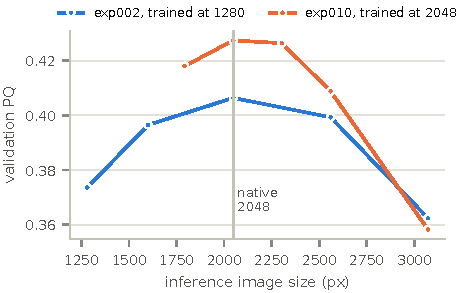
\includegraphics[width=0.66\textwidth]{figures/fig_resolution.pdf}
\caption{Validation PQ against the inference resolution, for a model trained at 1280 pixels (exp002)
and one trained at 2048 (exp010). Both peak at the native frame.
\generatedby{book/make\_book\_figures.py:fig\_resolution}}
\label{fig:yolo-resolution}
\end{figure}

Beyond the native size the score falls. At 3072 pixels SQ is essentially unchanged (0.6728, against
0.6695 at 2048), but RQ drops from 0.607 to 0.539: the masks that are found are no better, and fewer
of them are found. Enlarging an image adds no information that the camera did not record, and it
pushes the objects beyond the range of sizes that the detector learned.

Our first explanation of the peak was that a detector responds best to inputs about 1.6 times larger
than its training size, and $1.6\times1280=2048$. We tested this in exp024, using a model (exp010)
that had been trained at 2048 pixels, for which the explanation predicted a peak near 3300. The peak
was again at 2048. The simpler reading was the correct one: the peak occurs at the \emph{native
frame}, where every recorded pixel is present, and the factor of 1.6 was a coincidence.

\section{Masks that are too wide}\label{sec:yolo-erosion}
Our next experiment, exp005, was built on a hypothesis about thin structures. YOLO thresholds a
smooth mixture of prototypes at one half, so the edges of a thin ridge should be the first parts to
fall below the threshold. The masks should therefore be too \emph{thin}, and growing them by a pixel
should help. The measurement showed the opposite, consistently across the whole range of changes
(Figure~\ref{fig:yolo-erosion}).

\begin{figure}[t]
\centering
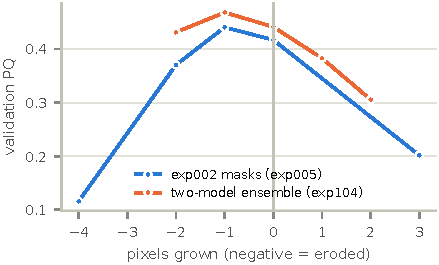
\includegraphics[width=0.66\textwidth]{figures/fig_erosion.pdf}
\caption{Validation PQ after a uniform change to every predicted mask, in pixels. Negative values
erode and positive values dilate. For the masks of exp002, and for the later two-model ensemble, one
pixel of erosion is best. \generatedby{book/make\_book\_figures.py:fig\_erosion}}
\label{fig:yolo-erosion}
\end{figure}

\begin{center}\small
\begin{tabular}{@{}cccccc@{}}
\toprule
pixels grown & PQ (confidence 0.35) & SQ & TP & FP \\
\midrule
$-4$ & 0.1156 & 0.595 & 200 & 535 \\
$-2$ & 0.3702 & 0.651 & 708 & 456 \\
$\mathbf{-1}$ & \textbf{0.4404} & \textbf{0.684} & 845 & 456 \\
$0$ & 0.4169 & 0.671 & 829 & 514 \\
$+3$ & 0.2016 & 0.602 & 448 & 905 \\
\bottomrule
\end{tabular}
\end{center}
Eroding every mask by one pixel, together with a confidence floor raised to 0.35, took the validation
score from 0.4064 to 0.4404 and the public score from 0.33 to 0.36. The optimum lies in the interior
of the grid in both directions: confidence thresholds of 0.30 and 0.40 are both worse, and so are
erosions of 0 and 2 pixels. The optimum is therefore not an artefact of where the grid
happened to end.

Two mechanisms were mixed together in this result. Erosion tightens masks that already match, but it
also shrinks marginal blobs below the minimum area of 300 pixels, so that they are dropped before
they can count as false positives. Repeating the sweep without the area filter separated the two.
The gain was $+0.0235$ with the filter and $+0.0223$ without it, so 95\% of it comes from correcting
the boundaries. SQ confirms this. It is the mean IoU over \emph{matched} pairs, so discarding
unmatched predictions cannot change it, and yet it rose from 0.6707 to 0.6837. Without the area
filter, erosion improved every count at once: true positives rose from 833 to 861, false positives
fell from 533 to 505, and false negatives fell from 492 to 464. This is the signature of a real
improvement to the boundaries. Near misses cross the IoU threshold of one half, and each crossing
turns one false positive and one false negative into one true positive
(Section~\ref{sec:metric-leverage}).

\subsection{Where the extra width came from}\label{sec:yolo-fat-cause}
Section~\ref{sec:masks-fat} traced the cause. Ultralytics draws its training targets with
\texttt{cv2.fillPoly}, whereas the competition scores with \texttt{pycocotools}. On filaments, which
consist mostly of boundary, the two conventions differ by about 11\% of the area. The model learns
the wider convention faithfully and reproduces it at test time.

One pixel of erosion over-corrects: it moves the area of the masks from about 11\% too large to
about 10\% too small. The two conventions differ by about half a pixel, and no operation on a binary
raster can remove half a pixel, because the distance transform of a binary mask takes only whole
steps. The proper fix works in coordinate space: shrink each polygon by 0.5 pixels before it is
rasterised (Listing~\ref{lst:masks-shrink}). This raised the agreement between the training targets
and the scorer's masks from an IoU of 0.898 to 0.959, and moved the ratio of their areas from 1.111
to 0.986. Every YOLO model that we trained afterwards used these corrected targets, and each of them
then performed best with \emph{no} erosion at test time, as one would expect if the targets were
right.

\subsection{Why the correction needs a full-resolution loss}\label{sec:yolo-maskratio}
The correction had a complication, caused by a setting of the library. Ultralytics builds its target
masks at the input size divided by a parameter called \texttt{mask\_ratio}, whose default value is 4,
and it computes the mask loss at that reduced size. At an input of 2048 pixels, the loss grid is
therefore only 512 cells wide, and a correction of half a pixel at 2048 amounts to an eighth of a
cell on the grid that the loss can see (Figure~\ref{fig:yolo-grid}). The correction almost vanishes
before the model is trained on it. The same is true of the error that the correction targets: 64\%
of the disagreement between predicted and annotated masks lies within two native pixels of the
boundary, which is half a cell at 512.

\begin{figure}[t]
\centering
\begin{tikzpicture}[scale=1.0]
  % (a) fine grid: loss at native resolution
  \begin{scope}
    \foreach \cx/\cy in {0/2, 1/2, 4/3, 7/4}
      \fill[vizorange!55] (\cx*0.25,\cy*0.25) rectangle ++(0.25,0.25);
    \draw[gridline, line width=0.4pt] (0,0) grid[step=0.25] (2,2);
    \draw[inkmuted, line width=0.6pt] (0,0) rectangle (2,2);
    \draw[vizblue, line width=1.1pt] (0,0.6) -- (2,1.2);
    \draw[vizblue, line width=1.1pt, dashed] (0,0.47) -- (2,1.07);
    \node[note] at (1,-0.35) {(a) loss on the native grid:\\ the offset flips four pixels};
  \end{scope}
  % (b) coarse grid: loss at a quarter of the resolution
  \begin{scope}[xshift=3.4cm]
    \draw[gridline, line width=0.4pt] (0,0) grid[step=1] (2,2);
    \draw[inkmuted, line width=0.6pt] (0,0) rectangle (2,2);
    \foreach \cx/\cy in {0.5/0.5, 1.5/0.5, 0.5/1.5, 1.5/1.5}
      \fill[inkmuted] (\cx,\cy) circle (1.2pt);
    \draw[vizblue, line width=1.1pt] (0,0.6) -- (2,1.2);
    \draw[vizblue, line width=1.1pt, dashed] (0,0.47) -- (2,1.07);
    \node[note] at (1,-0.35) {(b) loss on a 4$\times$ coarser grid:\\ no pixel centre moves side};
  \end{scope}
  \draw[vizblue, line width=1.1pt] (6.4,1.8) -- (6.9,1.8);
  \node[note, anchor=west] at (6.95,1.8) {annotated edge};
  \draw[vizblue, line width=1.1pt, dashed] (6.4,1.2) -- (6.9,1.2);
  \node[note, anchor=west] at (6.95,1.2) {edge moved inward by\\ half a native pixel};
  \fill[vizorange!55] (6.525,0.43) rectangle ++(0.25,0.25);
  \node[note, anchor=west] at (6.95,0.55) {pixel whose label\\ changes};
\end{tikzpicture}
\caption{Why a correction of half a pixel needs supervision at full resolution. On the native grid
(a), moving an edge inward by half a pixel changes the label of about one pixel in two along the
edge. On a grid four times coarser (b), the same move changes the side of almost no cell centre, so
the loss cannot see it. \drawnin{book/chapters/ch07\_yolo.tex}}
\label{fig:yolo-grid}
\end{figure}

Setting \texttt{mask\_ratio=1} makes the loss grid native. Besides its memory cost, this has a
subtler cost: a larger share of each mask's pixels lies in its interior, so the boundary receives
relatively less weight in the loss. For example, a filament of 1,275 pixels with a perimeter of 200
pixels has 15.7\% of its pixels on its rim at 2048, against about 62\% of its cells at 512. The trade
is nevertheless worth making, because the alternative is a loss that cannot represent the boundary
error at all.

\section{Retraining at native resolution}\label{sec:yolo-retrain}
Everything so far pointed to a single experiment: train at 2048 pixels, with the corrected targets
and \texttt{mask\_ratio=1}, until the training schedule has run to completion. Running that experiment
properly took five attempts and most of a week. We describe the attempts in turn, because each one
failed for a different reason, and several of the reasons recur in later chapters.

\subsection{exp010: two of three changes silently lost}\label{sec:yolo-exp010}
Experiment exp010 trained at 2048 pixels on a T4 GPU for Kaggle's twelve-hour limit. When we read
its configuration file afterwards, it said \texttt{mask\_ratio: 2}. The training script contained a
fallback ladder for memory errors, and when full-resolution supervision ran out of memory at batch
sizes 2 and 1, the script quietly moved to the third rung. At \texttt{mask\_ratio=2}, the half-pixel
correction is a quarter of a cell on the loss grid, so the corrected targets were again nearly
ineffective. In addition, the cosine learning-rate schedule~\citep{sgdr} had been sized for 400 epochs, and the
session reached only epoch 62. After twelve hours the learning rate was still 94\% of its peak value
of $10^{-3}$, so the model never went through the phase of low learning rates in which fine-tuning
earns much of its final accuracy. It scored 0.4274 on validation and 0.36 on the leaderboard.

\subsection{exp031: a completed schedule at 1536 pixels}\label{sec:yolo-exp031}
Experiment exp031 fixed both faults at the cost of some resolution: it trained at 1536 pixels, with
batch size 1, \texttt{mask\_ratio=1}, a frozen backbone, and 50 epochs of a cosine schedule that
annealed from $5\times10^{-4}$ to $5.5\times10^{-6}$. Getting it to run took five launches and two
wrong diagnoses. Freezing the backbone did not free the memory that we had expected it to free,
because the allocation that failed was a single tensor in the mask loss, whose size grows with the
number of filaments in the batch. This also explained why a single crowded photograph could end a
run five epochs after it started. A second problem was that several attempts made inside one
Python process produced byte-identical out-of-memory errors, because \texttt{torch.cuda.empty\_cache()} cannot
release memory that the previous trainer still references; running each attempt in a separate
process solved this. The run scored 0.4343 on validation and 0.36 on the leaderboard.

At this point four of our models, exp002, exp010, exp031 and a fusion of the first two, all appeared
on the leaderboard as 0.36. Their validation scores ranged from 0.4274 to 0.4411, a spread of 0.0137,
which is smaller than one step of the two-decimal leaderboard. Section~\ref{sec:val-transfer}
explains why differences of this size cannot be seen on the leaderboard, and why we needed a
different kind of change.

\subsection{exp067--exp073: native supervision that fits in memory}\label{sec:yolo-memory}
Why does the mask loss need so much memory? The answer is that every positive \emph{location}, not
every filament, expands a full-size target map and a full-size map of logits, and each filament has
up to ten positive locations (Section~\ref{sec:yolo-training}). The chunked mask loss in
\file{shared/chunked\_mask\_loss.py} processes the positive locations in small groups, and recomputes
each group during the backward pass instead of storing its intermediate results, a technique known as
\keyterm{activation checkpointing}~\citep{checkpointing}. This made \texttt{mask\_ratio=1} at 2048 pixels fit on a T4.

Its first run produced losses of NaN in 16-bit arithmetic, and the cause is worth recording. To keep
every parameter connected to the computational graph, the loss added the term
\texttt{proto.sum() * 0}. A sum over a large half-precision tensor can overflow to infinity, and
$\infty\times0$ is NaN. Connecting the parameters through a single element of the tensor, instead of
through its sum, fixed the problem, and we moved validation to 32-bit arithmetic. The model of exp068
then trained for five epochs (2.5 hours) and scored 0.4470 with test-time augmentation, below the
0.4586 of our best pipeline at that time.

The ROI loss in \file{shared/roi\_mask\_loss.py} made the same supervision nearly twice as fast,
using a simple observation from linear algebra. Upsampling is a linear operation, so for any
upsampling operator $U$ we have
\begin{equation}
U\Big(\sum_{j} c_{dj} P_j\Big) = \sum_{j} c_{dj}\, U(P_j).
\end{equation}
The standard loss first upsamples all 32 prototypes to the native size and then mixes them. The ROI
loss mixes them first, at a quarter of the resolution, which leaves a single map, and then samples
that map at the native resolution only inside the detection's box, using the differentiable
bilinear sampling of spatial transformer networks~\citep{jaderberg2015}
(Listing~\ref{lst:yolo-roi}). The
result is the same up to floating-point rounding, and the cost falls from 32 native-size maps per
image to one small map per detection.

\begin{lstlisting}[caption={A native-resolution mask loss evaluated only inside the box. Condensed
from \file{shared/roi\_mask\_loss.py}.},label=lst:yolo-roi]
def roi_mask_loss(coefficient, proto, truth, box, area, height, width):
    x0, y0, x1, y1 = box                                   # integer box at native resolution
    # mix FIRST: one low-resolution logit map instead of 32 upsampled prototypes
    low = (coefficient.float() @ proto.float().flatten(1)).reshape(1, 1, *proto.shape[-2:])
    # centres of the native pixels inside the box, in grid_sample's [-1, 1] coordinates
    x = (torch.arange(x0, x1, dtype=torch.float32) + 0.5) * (2 / width) - 1
    y = (torch.arange(y0, y1, dtype=torch.float32) + 0.5) * (2 / height) - 1
    yy, xx = torch.meshgrid(y, x, indexing="ij")
    grid = torch.stack([xx, yy], dim=-1)[None]
    logits = F.grid_sample(low, grid, mode="bilinear", padding_mode="border",
                           align_corners=False)[0, 0]    # same as upsample-then-crop
    return F.binary_cross_entropy_with_logits(logits, truth[y0:y1, x0:x1].float(),
                                              reduction="sum") / (height * width * area)
\end{lstlisting}

On the same crowded photographs, a full optimiser step took 1.58 seconds with the ROI loss and 2.86
seconds with the chunked loss, and peak memory fell from 9.4 to 5.9 GiB. Experiment exp073 continued
the training of exp068 with the ROI loss for four more epochs and reached 0.4555, still below 0.4586.

\subsection{exp097: a converged YOLOv8l-seg at 2048 pixels}\label{sec:yolo-exp097}
Our last YOLO run rented a 48 GB L40 GPU on RunPod at \$0.69 an hour, and trained the larger
YOLOv8l-seg at 2048 pixels, with the corrected targets, a batch size of 2, and full-resolution
supervision. Three engineering decisions defined the run.
\begin{enumerate}[leftmargin=*,itemsep=2pt]
\item \textbf{Its length was decided by convergence.} After the warm-up, the
learning rate stayed constant. When a three-epoch moving average of the validation fitness had not
improved by 0.002 for 12 epochs, the learning rate was multiplied by 0.2. After three such
reductions, a further plateau stopped the training (Algorithm~\ref{alg:yolo-plateau} and
Listing~\ref{lst:yolo-plateau}).
\item \textbf{Its batch size was measured.} A preflight step trained for a few iterations on the most
crowded images at each candidate batch size and chose the fastest one that fitted in memory. This was
a batch size of 2, which processed 9.4 images per second and used 39,396 of the GPU's 45,458 MiB.
\item \textbf{It was rehearsed on free hardware.} The second rented machine failed 35 seconds after
training began, because of a defect in our own callbacks. They had been written against an assumed
version of the Ultralytics API and tested only against that assumption. Reading the source code of
the pinned version of the library revealed four defects. After that, every payload was first run on
a free Kaggle T4 (exp099, with 23 automated checks) before any money was spent.
\end{enumerate}

\begin{algorithmblock}{Learning-rate decay on plateau, with stopping at convergence\label{alg:yolo-plateau}}
\item \textbf{parameters:} patience $n_p=12$ epochs, minimum improvement $\delta=0.002$, decay factor $0.2$, at most 3 decays
\item \textbf{after each epoch} (once the warm-up is over and three fitness values exist) \textbf{do}
\item \Ind $\bar f\leftarrow$ mean fitness of the last three epochs;
\item \Ind \textbf{if} $\bar f>f^{\ast}+\delta$ \textbf{then} $f^{\ast}\leftarrow\bar f$; reset the plateau counter; \textbf{continue};
\item \Ind increment the plateau counter; \textbf{if} it is below $n_p$ \textbf{then} \textbf{continue};
\item \Ind \textbf{if} fewer than 3 decays so far \textbf{then} multiply the learning rate by 0.2 and reset the counter;
\item \Ind \textbf{else} stop training: the model has converged at every learning rate tried
\end{algorithmblock}

\begin{lstlisting}[caption={Decay on plateau, stop at convergence. Condensed from
\file{experiments/exp\_097\_runpod\_yolo/src/convergence.py}.},label=lst:yolo-plateau]
def update(self, epoch, fitness):          # patience 12, min_delta 0.002, decay 0.2, 3 decays
    self.window.append(fitness)             # deque(maxlen=3): a moving average
    smoothed = sum(self.window) / len(self.window) if len(self.window) == 3 else None
    if epoch <= self.warmup_epochs or smoothed is None:
        return "continue"
    if self.best is None or smoothed > self.best + self.min_delta:
        self.best, self.best_epoch, self.since_best = smoothed, epoch, 0
        return "continue"                   # improved
    self.since_best += 1
    if self.since_best < self.patience:
        return "continue"                   # plateau, still counting
    if self.decays < self.max_decays:
        self.decays += 1; self.lr_scale *= self.decay_factor; self.since_best = 0
        return "decay"                      # every lower rate gets a full window
    return "stop"                           # converged at every rate tried
\end{lstlisting}

The run behaved as designed. The first stage reached a plateau and was decayed at epoch 75, and the
first decay lifted the fitness from 0.648 to 0.686 within six epochs. Training stopped at epoch 124
after three decays, having used learning rates of $10^{-3}$, $2\times10^{-4}$, $4\times10^{-5}$ and
$8\times10^{-6}$. The best fitness occurred at epochs 86 to 88, and the final mask mAP50 was 0.704.
The run cost \$2.74.

Scored with our own pipeline, the best checkpoint reached 0.4668 with test-time augmentation, which
made it the best YOLO model we produced. It appeared on the leaderboard as 0.39. Two further findings
came with it. First, the checkpoints saved at the second and third decays contained exactly the same
weights as the best checkpoint, because nothing after epoch 88 improved the fitness; the last 36
epochs bought nothing. Second, the checkpoint from the end of the first stage, whose fitness was
only 0.047 lower, scored just 0.4538. Fitness measures ranking, whereas PQ measures a single emitted
set, and the relationship between the two is not constant.

\section{What the YOLO models could and could not do}\label{sec:yolo-lessons}
The YOLO models took the public score from 0.32 to 0.39, through inference at the native resolution,
corrected targets, test-time augmentation (Chapter~\ref{ch:tta}) and ensembles. A converged model,
trained at the native resolution with correct targets and full-resolution supervision, still
appeared as 0.39, and we did not find a way to take this family further.

A public notebook from a team with a leaderboard score of about 0.55 runs YOLOv8l-seg at 2048 pixels
with a confidence floor of 0.30. It contains a defect: it orders overlapping masks by their class
index, which is zero for every mask, instead of by their confidence. In exp095 we ran the notebook's
inference procedure on our own weights from exp002 (YOLO11m-seg trained at 1280 pixels). It scored
0.4111, against 0.4469 for our best single-view procedure on the same weights. If that team's
advantage is real, it must therefore lie in its trained model rather than in its inference
procedure. Our own
YOLOv8l-seg, trained at the same resolution to convergence, appeared as 0.39, and we never explained
the gap.

Ultralytics also taught us to distrust configuration. The library changes what one asks for without
failing, and each of the following behaviours affected one of our runs.
\begin{itemize}[leftmargin=*,itemsep=1pt]
\item With \texttt{optimizer="auto"}, the library ignores \texttt{lr0} and chooses its own optimiser
and learning rate.
\item A bare \texttt{resume=True} searches the library's own settings folder for a run to resume,
and ignores the folder of the current project.
\item Removing the \texttt{time=} argument also removes the rescaling of the learning-rate schedule
to the time budget.
\item Setting \texttt{augment=True} on a segmentation model logs a warning and runs at a single
scale.
\item An out-of-memory error in the first epoch halves the batch size and rebuilds the optimiser.
\end{itemize}
The defence is to read back the resolved configuration of every run (the file \file{args.yaml}),
and to check the learning rate that the optimiser actually uses rather than the one that was
passed to it.

Finally, the question raised in Section~\ref{sec:yolo-prototypes}, whether the 32-prototype basis
limits the masks, was never settled cleanly. The most direct test, a converged model at the native
resolution, gained 0.011 on validation over our standing baseline. This was neither the collapse nor
the leap that would have answered the question. What the YOLO experiments did establish is that no
further gain of the size we needed was available from this family of models, and this led us to a
model that predicts each mask from its own query (Chapter~\ref{ch:transformers}).

\section*{Exercises}
\begin{exercise}{The size of the basis}
A mask in Equation~\eqref{eq:yolo-mask} is a thresholded combination of 32 maps at a quarter of the
resolution. Take one annotated filament, downsample its mask by a factor of 4, and fit the best
combination of 32 smooth random maps to it (least squares on the logits). How does the IoU of the
reconstruction depend on the width of the filament? Compare a thin filament with a thick one.
\end{exercise}

\begin{exercise}{Why the threshold sweep is flat}
Using the first and last rows of the threshold table in Section~\ref{sec:yolo-exp002}, compute the
change in the numerator and in the denominator of PQ between the confidence thresholds 0.30 and
0.20. Explain why 59 extra true positives bought nothing.
\end{exercise}

\begin{exercise}{Counting flipped pixels}
In Figure~\ref{fig:yolo-grid}, an edge moves inward by half a native pixel. Show that on a grid whose
cells are $s$ native pixels wide, the expected fraction of cells along the edge whose centres change
side is $\min(1, 0.5/s)$. Evaluate this fraction for \texttt{mask\_ratio} values of 1, 2 and 4 at an
input size of 2048.
\end{exercise}

\begin{exercise}{Linearity of upsampling}
Prove that bilinear interpolation is a linear operator. Then verify numerically that
Listing~\ref{lst:yolo-roi} gives the same logits as upsampling all 32 prototypes with
\texttt{F.interpolate(..., mode="bilinear", align\_corners=False)} and then cropping.
\end{exercise}

\begin{exercise}{A controller on a noisy curve}
Simulate fitness curves as a saturating function of the epoch plus Gaussian noise with a standard
deviation of 0.01. Run Algorithm~\ref{alg:yolo-plateau} on them, and measure how often it decays too
early as the length of the moving-average window changes from 1 to 5.
\end{exercise}
